%First stage



\begin{figure}[htbp]
    \centering
    
    \begin{subfigure}{\textwidth}
        \centering
        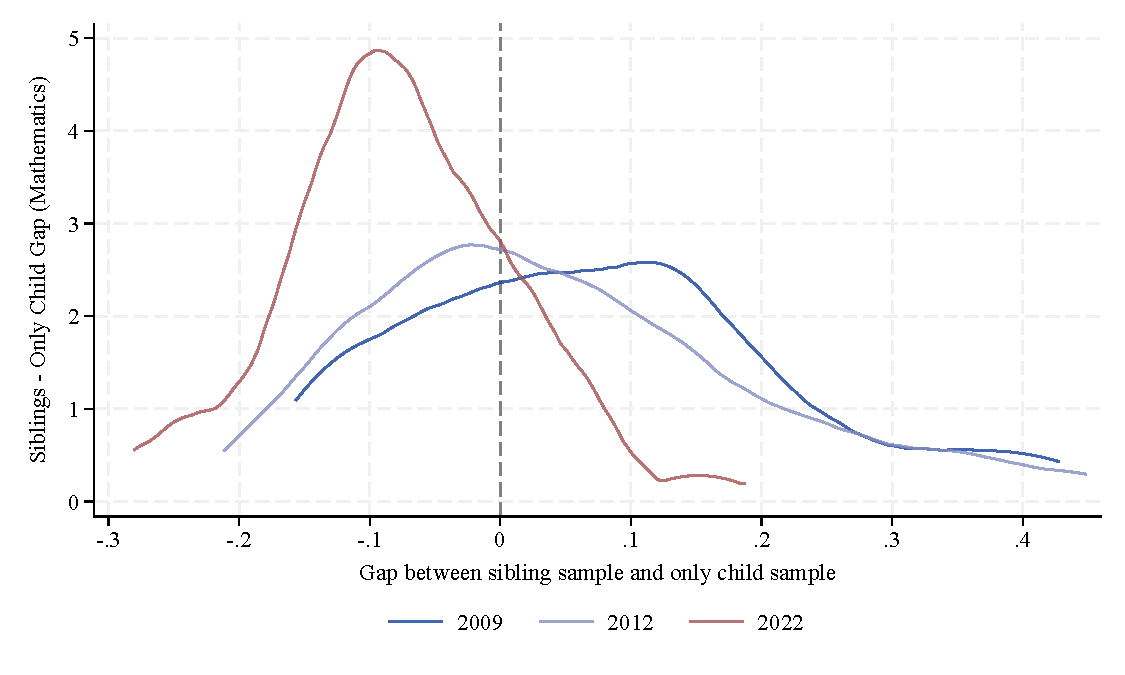
\includegraphics[width=\textwidth]{./FIGURES/Descriptive/PISA_gap_PV1MATH_histogram_2009_2022.pdf}
        \caption{Learning gaps in Mathematics by year}
        \label{fig:1a}
    \end{subfigure}
    
    \vspace{1em} % Add some vertical space between subfigures
    
    \begin{subfigure}{\textwidth}
        \centering
        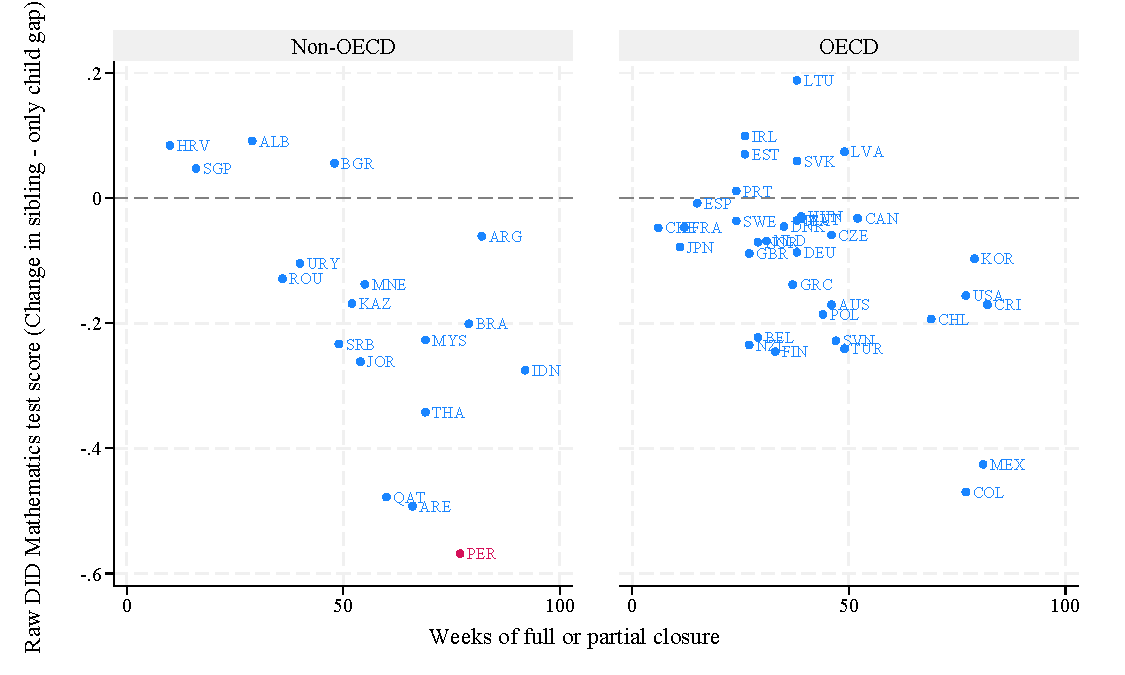
\includegraphics[width=\textwidth]{./FIGURES/Descriptive/PISA_raw_DID_PV1MATH_not_fully_open.pdf}
        \caption{Change in learning gaps by duration of school closure for OECD and Non-OECD countries.}
        \label{fig:1b}
    \end{subfigure}
    
    \caption{Learning gaps around the world}
    \label{fig:combined}
\end{figure}


\begin{figure}[htbp]
    \centering
    
    \begin{subfigure}{\textwidth}
        \centering
        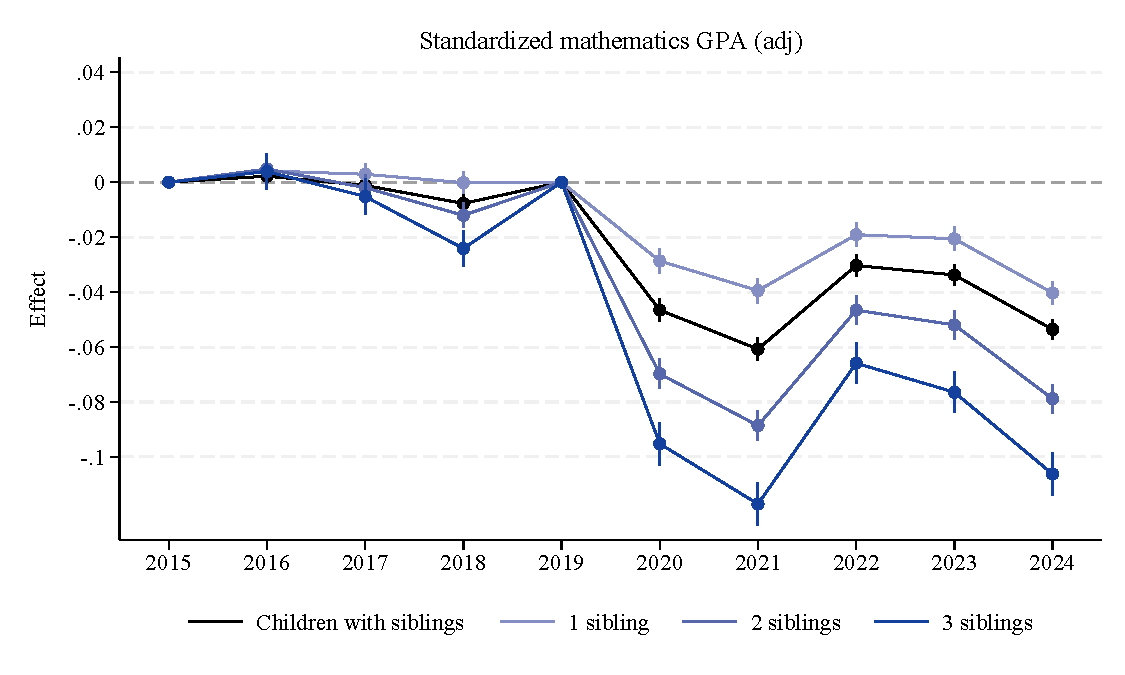
\includegraphics[width=\textwidth]{./FIGURES/Event Study/covid_std_gpa_m_adj_all_all_all_elm_all.pdf}
        \caption{Event Study}
        \label{fig:1a}
    \end{subfigure}
    
    \vspace{1em} % Add some vertical space between subfigures
    
    \begin{subfigure}{\textwidth}
        \centering
        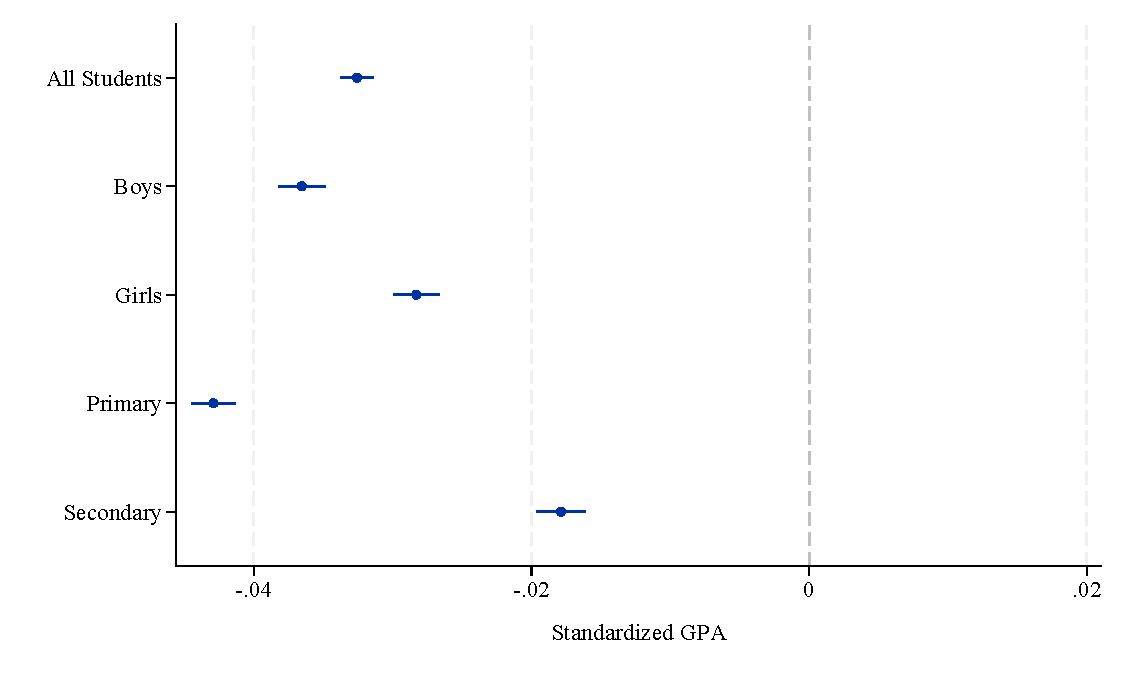
\includegraphics[width=\textwidth]{./FIGURES/TWFE/covid_twfe_B_all_all_gpa_m_adj_4.pdf}
        \caption{Change in gap between children with siblings and only childs}
        \label{fig:1b}
    \end{subfigure}
    
    \caption{Learning gap between only childs and siblings}
    \label{fig:combined}
\end{figure}


\clearpage

%RD-first grade
\makeatletter
\@ifclassloaded{beamer}{%
       \centering
       \resizebox{0.6\textwidth}{!}%
}{%
       \begin{table}[!tbp]\centering\def\sym#1{\ifmmode^{#1}\else\(^{#1}\)\fi}
       \centering
       \caption{Effects of younger sibling delaying school on older sibling standardized exams - 1 - m - a -  - 365}
       \label{tab:rd_summ_1_m_a_365}
       \resizebox{0.95\textwidth}{!}%
}
{
\makeatother
\resizebox{\textwidth}{!}{
\begin{tabular}{lccc}
\toprule
\cmidrule(lr){2-4}
& \multicolumn{3}{c}{Standardized GPA} \\
\cmidrule(lr){2-4}
& Pre-Covid & Covid & Post-Covid  \\
& 2018-2019 & 2020-2021 & 2022-2023  \\
\cmidrule(lr){2-2} \cmidrule(lr){3-3} \cmidrule(lr){4-4}
& (1) & (2) & (3)  \\
\bottomrule
&  &  &   \\
\multirow{2}{*}{\shortstack[l]{Younger sibling born after \\ school-entry cutoff}}&      -0.023***&      -0.001   &      -0.023***\\
                    &     (0.007)   &     (0.007)   &     (0.006)   \\
Local Linear        &         Yes   &         Yes   &         Yes   \\
                    &               &               &               \\
Observations        &     358,861   &     354,044   &     447,536   \\
Counterfactual mean &       0.058   &       0.020   &       0.050   \\
Bandwidth           &         365   &         365   &         365   \\
 

\bottomrule
\end{tabular}
}
\@ifclassloaded{beamer}{%
}{%
       \end{table}
}




